
%(BEGIN_QUESTION)
% Copyright 2010, Tony R. Kuphaldt, released under the Creative Commons Attribution License (v 1.0)
% This means you may do almost anything with this work of mine, so long as you give me proper credit

Determine the new positions of the water columns in water manometer, once an air pressure of 0.25 PSIG is applied to the right-hand tube.  The manometer is currently drawn as it would be in a condition of rest (no applied pressure).  Assume the scale is calibrated in {\it inches}, with marks above the zero line being positive and marks below the zero line being negative:

$$\includegraphics[width=15.5cm]{i03575x01.eps}$$

Height of water column registered in left-hand tube = \underbar{\hskip 50pt} inches

\vskip 10pt

Height of water column registered in right-hand tube = \underbar{\hskip 50pt} inches

\underbar{file i03575}
%(END_QUESTION)





%(BEGIN_ANSWER)

\noindent
5 points each answer:

\vskip 10pt

Height of water column registered in left-hand tube = \underbar{\bf +3.46} inches

\vskip 10pt

Height of water column registered in right-hand tube = \underbar{\bf -3.46} inches

\vskip 10pt

Deduct 2 points if the second answer is shown lacking a negative sign.

%(END_ANSWER)





%(BEGIN_NOTES)

{\bf This question is intended for exams only and not worksheets!}.

%(END_NOTES)


